\documentclass[sigconf]{acmart}
\usepackage[utf8]{inputenc}
\usepackage{booktabs} % For formal tables
\usepackage{balance} % For balanced columns on the last page
\usepackage{subcaption}
\usepackage{graphicx}
\usepackage{booktabs}
\usepackage{tablefootnote}

\copyrightyear{2019} 
\acmYear{2019} 
\setcopyright{acmcopyright}
\acmConference[MobileApps 2019]{Building Web and Mobile Apps 2019}{Winter term 2018/2019}{Fulda, Germany}
\acmBooktitle{MobileApps 2019: Building Web and Mobile Apps 2019, winter term 2018/2019, Fulda, Germany}
\acmPrice{0.00}
%\acmDOI{0}
%\acmISBN{0}

% Use the "authoryear" citation style, and make sure citations are in [square brackets].
\citestyle{acmauthoryear}
\setcitestyle{square}

% A useful command for controlling the number of authors per row.
% The default value of "authorsperrow" is 2.
\settopmatter{authorsperrow=0}

% end of preamble.

\begin{document}

% Title. 
% If your title is long, consider \title[short title]{full title} - "short title" will be used for running heads.
\title[Unity Mobile Games]{Improving the performance of Unity mobile games}

% Authors.
\author{Dan-Andrei Iorga 1154111}
\affiliation{
  \institution{Fulda University of Applied Sciences}
  \streetaddress{Leipziger Stra{\ss}e 123}
  \postcode{36037} 
  \city{Fulda} 
  \country{Germany}
}
\email{dan-andrei.iorga@informatik.hs-fulda.de}


% This command defines the author string for running heads.
\renewcommand{\shortauthors}{A. Iorga}

% abstract
\begin{abstract}
Game engines such as Unity are convenient ways to center the development process on the game behaviour itself rather than hardware-level implementations. While they are powerful tools that can increase the productivity of the developers, this comes at the cost of efficiency. Ways must be devised to mitigate the performance loss of a premade engine to acceptable results. This paper will present the study of a sample game implemented in Unity and the results of applying various perfromance-improving techniques on it.
\end{abstract}

%
% The code below should be generated by the tool at
% http://dl.acm.org/ccs.cfm
% Please copy and paste the code below.
%

\keywords{
	Unity, 
	Game engines, 
	Games, 
	Mobile Applications,
	Mobile Games,
	Android, 
	Game development, 
	Application performance
}


% A "teaser" figure, centered below the title and authors and above the body of the work.
\begin{teaserfigure}
  \centering
  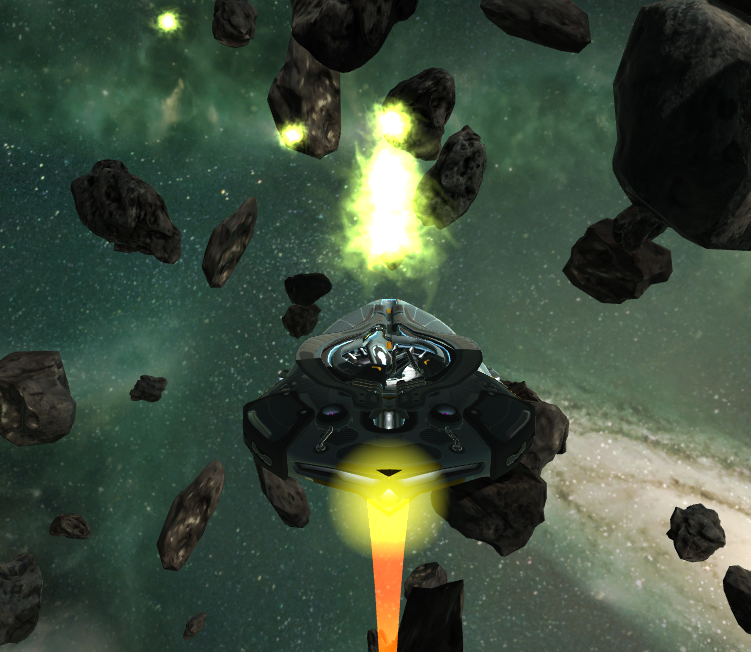
\includegraphics[width=\linewidth]{images/teaser}
  \caption{Space Shooter screenshot}
  \label{fig:teaser}
  \vspace{0.03cm}
\end{teaserfigure}
% Processes all of the front-end information and starts the body of the work.
\maketitle
\section{Introduction}
Lorem ipsum dolor sit amet, consectetur adipiscing elit. Vestibulum nisl ante, commodo non ligula non, ultrices mollis ante. Mauris dignissim justo a nibh vestibulum consectetur. Aenean sollicitudin, turpis ac fringilla cursus, nulla quam scelerisque est, at blandit ex felis in urna. Fusce in quam eleifend odio dignissim mollis. Aliquam eleifend lectus massa, ac vestibulum tellus ullamcorper eget. Proin lacus eros, tempor ac elementum a, tempus eu urna. Vestibulum vitae eros ac nulla placerat elementum nec sed tortor. Sed in urna metus. Praesent quis nisl nisi. Duis pharetra risus sed bibendum molestie. Aliquam nunc augue, finibus a diam ac, dignissim porttitor est.
Lorem ipsum dolor sit amet, consectetur adipiscing elit. Vestibulum nisl ante, commodo non ligula non, ultrices mollis ante. Mauris dignissim justo a nibh vestibulum consectetur. Aenean sollicitudin, turpis ac fringilla cursus, nulla quam scelerisque est, at blandit ex felis in urna. Fusce in quam eleifend odio dignissim mollis. Aliquam eleifend lectus massa, ac vestibulum tellus ullamcorper eget. Proin lacus eros, tempor ac elementum a, tempus eu urna. Vestibulum vitae eros ac nulla placerat elementum nec sed tortor. Sed in urna metus. Praesent quis nisl nisi. Duis pharetra risus sed bibendum molestie. Aliquam nunc augue, finibus a diam ac, dignissim porttitor est.
Lorem ipsum dolor sit amet, consectetur adipiscing elit. Vestibulum nisl ante, commodo non ligula non, ultrices mollis ante. Mauris dignissim justo a nibh vestibulum consectetur. Aenean sollicitudin, turpis ac fringilla cursus, nulla quam scelerisque est, at blandit ex felis in urna. Fusce in quam eleifend odio dignissim mollis. Aliquam eleifend lectus massa, ac vestibulum tellus ullamcorper eget. Proin lacus eros, tempor ac elementum a, tempus eu urna. Vestibulum vitae eros ac nulla placerat elementum nec sed tortor. Sed in urna metus. Praesent quis nisl nisi. Duis pharetra risus sed bibendum molestie. Aliquam nunc augue, finibus a diam ac, dignissim porttitor est.
Lorem ipsum dolor sit amet, consectetur adipiscing elit. Vestibulum nisl ante, commodo non ligula non, ultrices mollis ante. Mauris dignissim justo a nibh vestibulum consectetur. Aenean sollicitudin, turpis ac fringilla cursus, nulla quam scelerisque est, at blandit ex felis in urna. Fusce in quam eleifend odio dignissim mollis. Aliquam eleifend lectus massa, ac vestibulum tellus ullamcorper eget. Proin lacus eros, tempor ac elementum a, tempus eu urna. Vestibulum vitae eros ac nulla placerat elementum nec sed tortor. Sed in urna metus. Praesent quis nisl nisi. Duis pharetra risus sed bibendum molestie. Aliquam nunc augue, finibus a diam ac, dignissim porttitor est.
\section{Unity games}
\subsection{Game components}
It is important to draft an overview of the game before starting implementation, just like any other piece of software. The first question is whether the game should be 2D or 3D, as this would result in a vastly different game between the 2 choices, even if the main concepts stay the same. There are also hybrid options, such as Ortographic 3D or 2D gameplay with 3D graphics (also referred to as 2.5D), where 3D-based physics would serve a more aesthetic than functional role. The sample game used and developed in this study is a fully 3D game.\\
Another critically important choice is the genre of the game, which helps define the game world. The game world is where everything happens, it is what the player will see, the objects the player character interacts with and where the scope and purpose of the game exist. Essentially, the game world is to the player character as the real world is to the actual player. Main aspects to consider here would be for example whether the game would be a strategy-based game, in which case the player would control an array of game objects (often referred to as units), or a role-playing / shooting game, where typically the control of a single player character of a time is involved. This also impacts the User Interface within the game, as player controls and game information are closely related to the genre. \\ \\
\begin{figure}
\centering
\begin{subfigure}{0.49\textwidth}
\begin{subfigure}{0.49\textwidth}
\centering
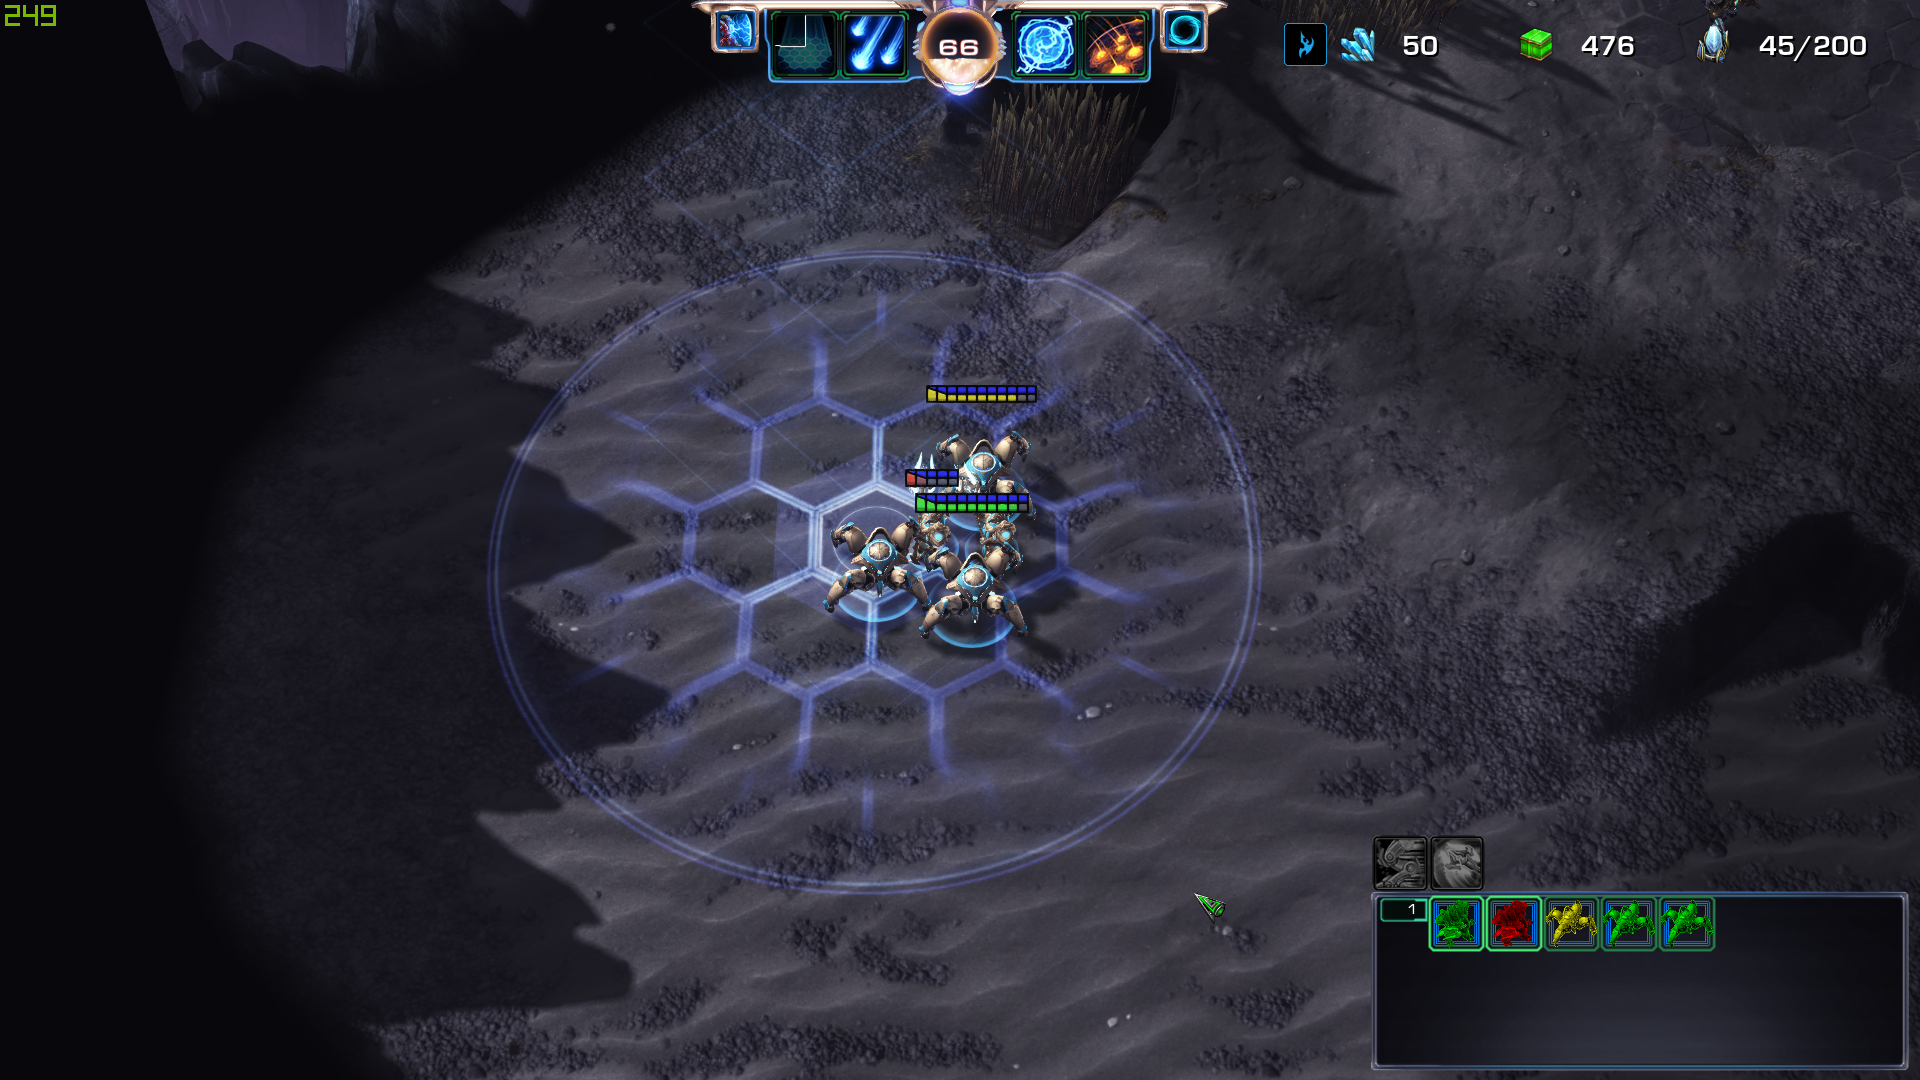
\includegraphics[width = \textwidth, height = 0.66\textwidth]{images/sc2}
\caption{Strategy game - Starcraft II (Blizzard Entertainment)}
\label{fig:left}
\end{subfigure}
\begin{subfigure}{0.49\textwidth}
\centering
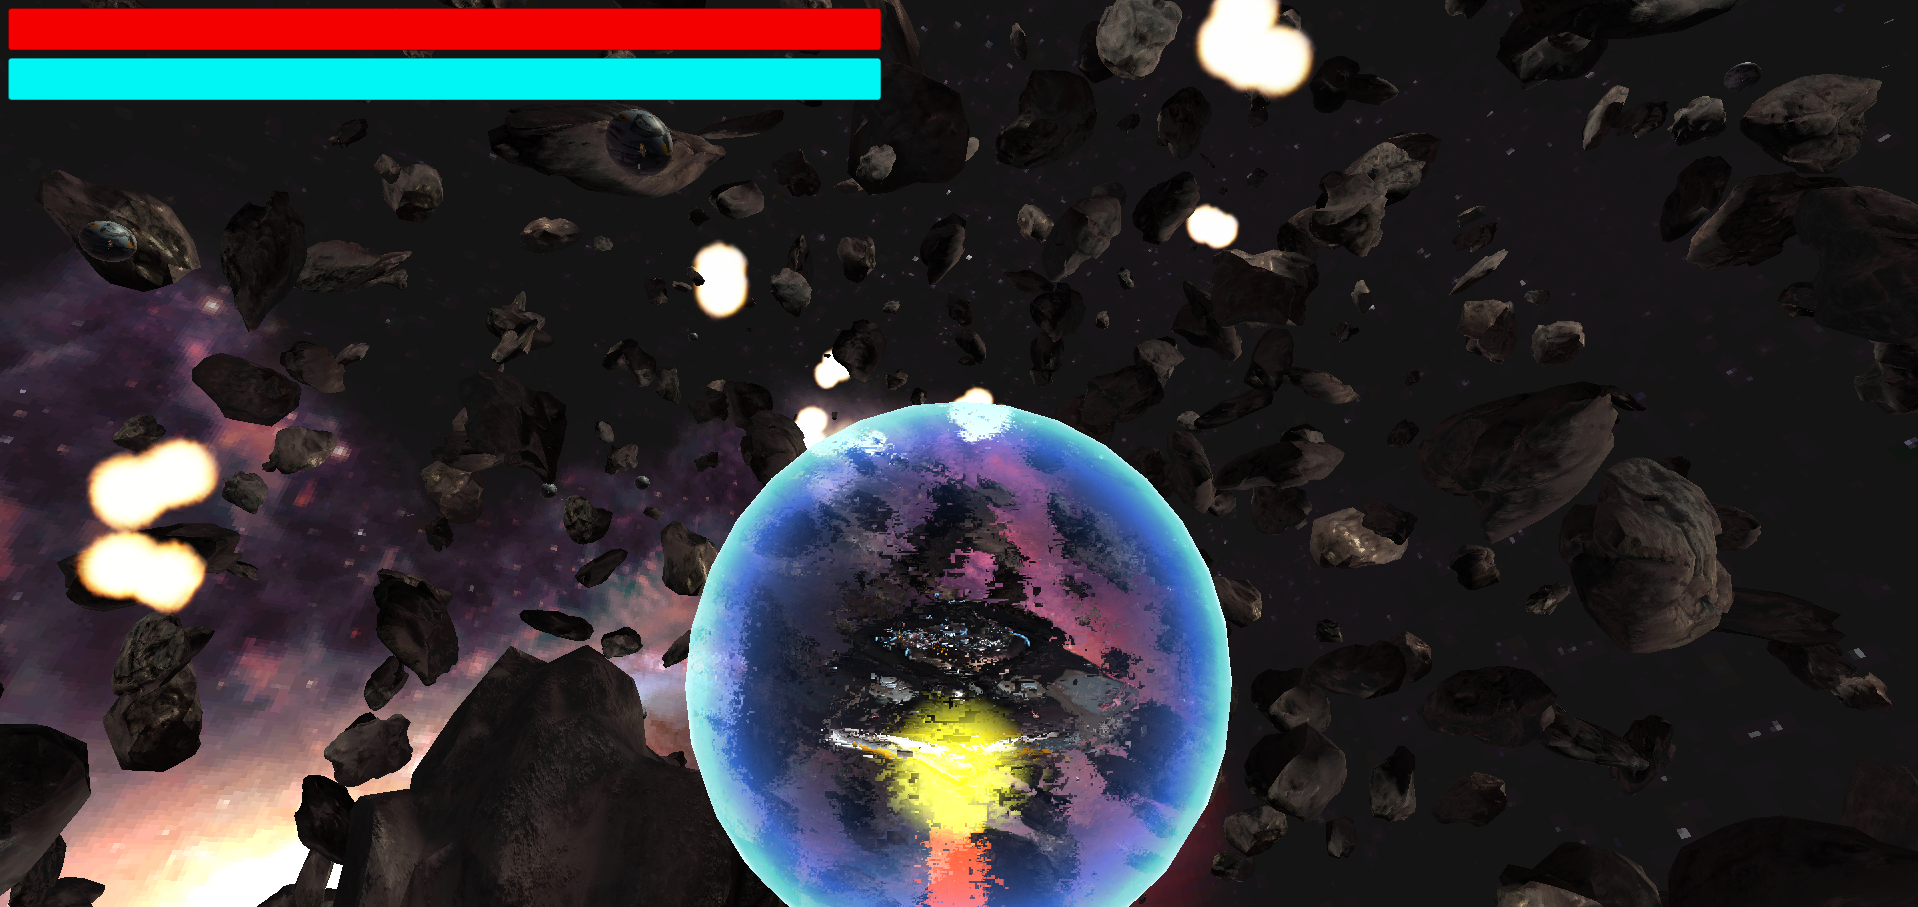
\includegraphics[width = \textwidth, height = 0.66\textwidth]{images/spaceshooter}
\caption{Space Shooter game - sample game}
\label{fig:right}
\end{subfigure}
\end{subfigure}
\caption{Strategy and Shooting genres first impression}
\label{fig:combined}
\end{figure}
In Figure 2.a, an example of a Strategy game is shown. The camera angle is worth noting, as it is not moving along with the controlled game objects, instead it is controlled manually by the player at will. In Figure 2.b, the sample game developed for this paper is shown. The camera cannot be directly controlled, instead it follows the player character, the ship, as it flies around. \\ \\
On paper, the game world is limited by the creator's imagination. In practice however, it is limited by the development possibilities, resources and hardware. Every object present in the game must be modeled (whether 3D or 2D), art, effects, behaviors, animations, everything must be created from scratch. Unity also provides developers with an Asset Stores where content creators can make their works available (free or paid) for others to use, but in the end, everything is made from scratch. The more work and objects are put in the game world, the richer it becomes, but this comes with a penalty in performance. Every object, effect, or behavior comes with its cost, which may be greater or smaller. Once the limit of hardware is reached, compromises must be made, such as limiting the game world in some way, or raising the target hardware performance. Each option has its drawbacks, players may be less interested in a game that doesn't look ``as pretty'', and likewise may not be interested in a game that requires too expensive hardware to be playable. In the strategy genre for example, the mechanic of the player creating more units is often encountered. A limit to the number of units should be implemented, or the game's performance will steadily decrease as more units are added.\\ \\
The player can see the game world through the use of cameras, which render parts of the world, translating a 3D environment (if necessary) to a flat, 2D image. This image can be either displayed on the screen, often called the main camera, or used as a texture for effects such as in-game computer screens displaying other areas of the game world.\\
Textures are essentially object skins. They are wrapped around them, stretching to match certain texture mapping points on them. The end result is a finished object, with the shape of the model and the coloring of the texture, as it is mapped.\\
Another key aspect in a game is the lighting system. Without light, there is nothing to see, resulting in a disappointing experience for the player. Shadows and reflections bring realism, by altering the effect light has on various object to emulate real world effects. In 3D rendering, two major techniques are used: rasterization and ray-tracing. \\
The most widely used is rasteriztion, a highly efficient method that trades fidelity for speed, often with results that fool the user into not noticing the visual anomalies. ``With rasterization, objects on the screen are created from a mesh of virtual triangles, or polygons, that create 3D models of objects. In this virtual mesh, the corners of each triangle — known as vertices — intersect with the vertices of other triangles of different sizes and shapes. A lot of information is associated with each vertex, including its position in space, as well as information about color, texture and its “normal,” which is used to determine the way the surface of an object is facing.
Computers then convert the triangles of the 3D models into pixels, or dots, on a 2D screen. Each pixel can be assigned an initial color value from the data stored in the triangle vertices.
Further pixel processing or “shading,” including changing pixel color based on how lights in the scene hit the pixel, and applying one or more textures to the pixel, combine to generate the final color applied to a pixel.'' \cite{NvidiaRastRT} \\
Another important piece of a well-made Unity game is it's scripting system. The language of choice for them is either Javascript or C\#, the latter being used for the Space Shooter game. Scripts define behaviors and interactions between various game objects, being able to manipulate, create and destroy them.  \\
Player interaction is done through the UI, using buttons, canvases, progress bars, key presses and other similar means. Those components do not directly interact with other game objects, but may have effects on the game world through scripts attached. \\ \\
The vibrancy and the ability to captivate a player lies in the effects, providing immersion. Sound effects played at key moments, particle systems making trail, smoke and explosion effects, all these serve to improve the quality of the player experience, but again, at a cost of performance. Particle systems create many automatically managed, low impact game objects (particles), but when used too often, and with too high particle count, it can affect the smoothness of the gameplay, something undesirable for any player. \\
Unity provides a plethora of features and options, many being outside the scope of this paper. The reader is encouraged to check the Unity official documentation for further study. \cite{unitymanual}
\subsection{Games vs Hardware}
Video games can be very computationally intensive. Certain tasks rely on the machine's CPU power (script execution, physics, game object search/creation), others on the GPU (lighting, texture processing, camera rendering). Different platforms have different specs, with great possible deviations from the average. The processing power of some devices can be strongly imbalanced towards the CPU, providing only minimal support for graphics. \\ \\
Unity provides great resource usage data to track which part of the hardware is most taxed, which is often the best place to start optimizing. The Breakdown View can be used to see the call stacks on the CPU and GPU, see which tasks take the most, keep track of memory usage and thus identify which elements have the highest negative impact. \\ \\
Most often, the cause of low performance is suboptimal usage of the CPU and/or system memory by the MonoBehaviour, the base class for any script attached to game objects, or the physics/collision systems. As far as the GPU is concerned, prime exampled would be the needless usage of high-resolution texture, too many/intense particle systems or the use of high-fidelity rendering techniques such as ray tracing. The target rendering resolution also plays an important role as far as GPU loads are concerned.
\subsection{Game platforms}
\begin{table*}[t]
\caption{Gaming platform specs}
\label{tab:conf}
\begin{minipage}{\textwidth}
\begin{center}
\begin{tabular}{lllllll}
Component & Xbox One X & iPad Pro 11 & Moto E 4 & Custom-built PC & Low-end Laptop \\
CPU\footnote{Number of threads derived from core count and hyperthreading availability} & 8T x86 2.3 Ghz & 8T Apple A12X 2.26 Ghz & 4T ARM-A53 1.1 Ghz & 12T Intel 4.7 Ghz & 4T Intel 2.2Ghz \\
GPU & Integrated AMD & PowerVR 7XT & ARM Mali-T720 & Nvidia RTX 2080Ti & Nvidia GT 940m \\
GPU Compute power & 6 TFLOPs &  Not available &  Not available & 13.4 TFLOPs & 0.9 TFLOPs \\
RAM & 12 GB & 4 GB & 2 GB  & 32 GB & 8 GB \\
VRAM & 12 GB & Not available &  Not available & 11 GB & 2 GB \\
VRAM Type\footnote{Shared VRAM systems show the total value for both RAM and VRAM} & Shared &  Not available &  Not available & Dedicated & Dedicated \\
Storage & 1TB & 1TB\footnote{From 64 GB up to 1 TB} & 16 GB & 1.25 TB & 625 GB
\end{tabular}
\bigskip
\footnotesize\emph{Note:} Specs taken via official product pages. \\
\emph{Source:}\cite{rtxspecs} \cite{motospecs} \cite{xboxspecs} \cite{laptopspecs} \cite{intelspecs} 
\end{center} 
\end{minipage}
\end{table*}
As previously stated, Unity supports over 25  different platforms across mobile, desktop, TV, AR/VR and Web. In this paper we will focus our attention on PC and Android devices, PC because it is already the development environment for our sample game, and Android because of device availability as far as mobile platforms are concerned. This section will show a brief overview of various platforms and specs across the mainstream gaming choices, console, mobile and PC. \\ \\
The fine differences between all the platforms and devices belonging in each are beyond the scope of this study, however, after just a glance (see Table 1), it is clear and reasonable that mobile devices are not dedicated gaming machines, falling short when compared to dedicated machines made for gaming (consoles such as the Xbox One X) or custom built PC's. This serves as a strong argument that great care must be taken when developing mobile games, as the mobile platform has many limitations imposed due to the very nature of the hardware used (thermal values, power, computational power, system resources). Naturally, there are other options beyond the three platforms depicted here, but since the main focus here is mobile development, going into more detail regarding all platforms proves to be extraneous.
\subsection{Space Shooter}
The Space Shooter game, as the name suggests, is a generic implementation of the space shooter genre. It involves the player flying a ship through (relatively) open space and interacting with various space bodies present. These spacial bodies may be passive, friendly or hostile. \\ 
This game was developed specifically to showcase the concepts discussed in this study, and thus lacks certain details that were deemed irrelevant to the discussed topic. The following sections will describe the Space Shooter game  more in-depth.
\subsubsection{Game description}
As previously stated, the game belongs to the space shooter genre. Such games involve the control of a space ship, flying in a two-dimensional or three-dimensional space, avoiding collisions with other spatial bodies by dodging or shooting the ship weapon(s) at the targets. Generally, such a game includes ``life'' mechanics, such that the player ship will eventually be destroyed and the game ended upon taking too much damage. \\ \\
Because the purpose of this game is purely demonstrative with regard to performance optimization techniques, certain irrelevant or negligible components are missing. As such, the game has no clearly defined goal / victory conditions, nor does it implement any game control mechanics beside a simple defeat screen. The game also does not have any sound effect, as a full study on all features present in Unity would not be feasible in the context of this study. Menus are limited to the defeat screen, enabling the player to restart the game. \\ \\
The game assets (models, textures, effects) have been either made from scratch, imported from the Asset Store with usage rights or imported and modified.
\begin{figure}
\centering
\begin{subfigure}{0.49\textwidth}
\centering

\begin{subfigure}{0.49\textwidth}
\centering
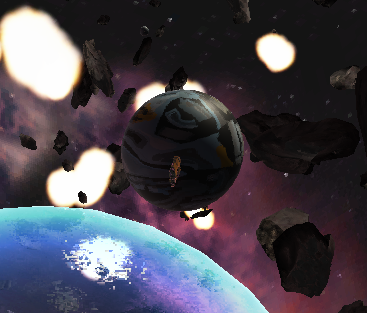
\includegraphics[width = \textwidth, height=\textwidth]{images/game1}
\caption{Space Drone - hostile}
\label{fig:top}
\end{subfigure}
\begin{subfigure}{0.49\textwidth}
\centering
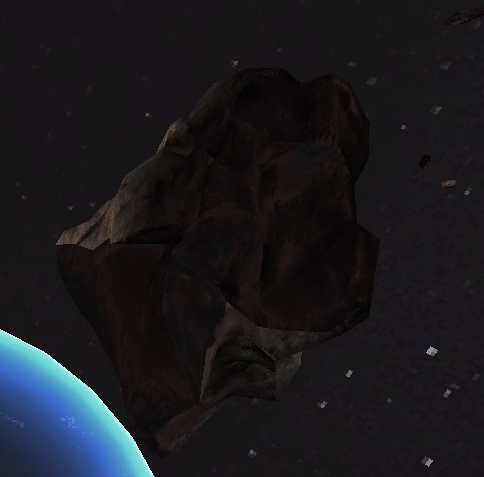
\includegraphics[width = \textwidth, height=\textwidth]{images/game2}
\caption{Space Asteroid - passive}
\label{fig:bottom}
\end{subfigure}

\label{fig:left}
\end{subfigure}
\begin{subfigure}{0.49\textwidth}
\centering

\begin{subfigure}{0.49\textwidth}
\centering
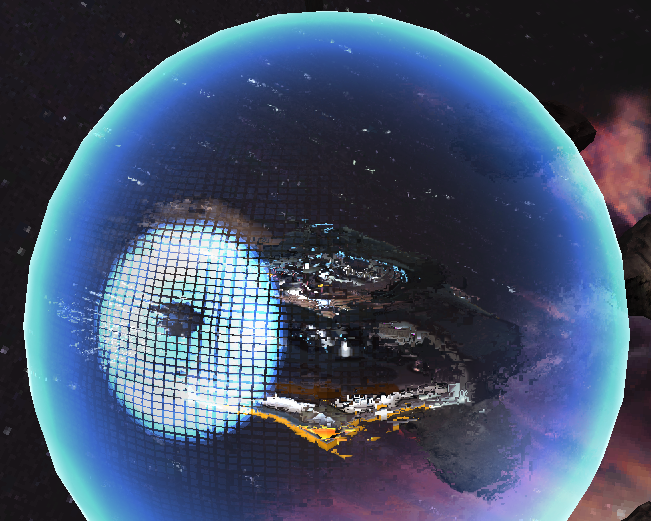
\includegraphics[width = \textwidth, height=\textwidth]{images/game3}
\caption{Player ship}
\label{fig:top}
\end{subfigure}
\begin{subfigure}{0.49\textwidth}
\centering
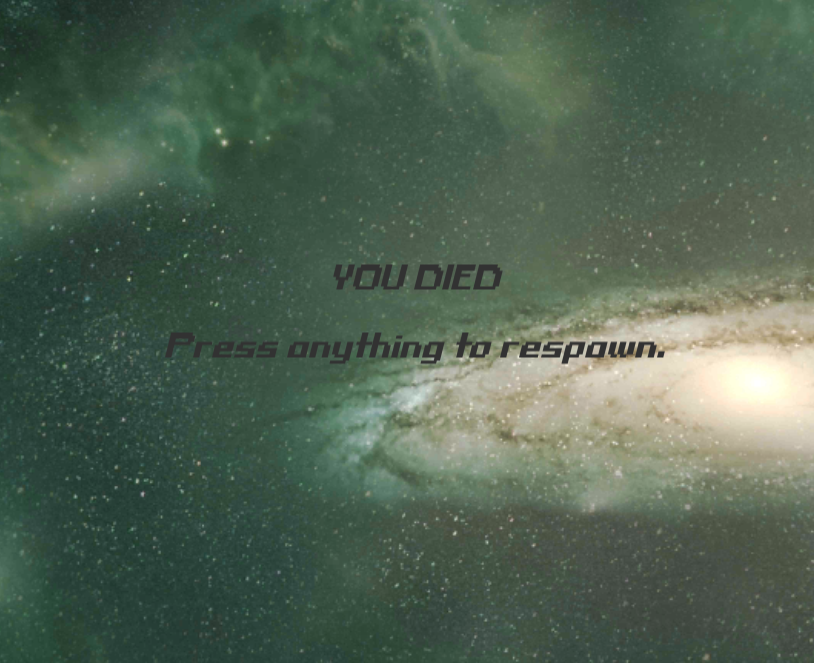
\includegraphics[width = \textwidth, height=\textwidth]{images/game4}
\caption{Defeat screen}
\label{fig:bottom}
\end{subfigure}

\label{fig:right}
\end{subfigure}
\caption{Space Shooter in a nutshell}
\label{fig:combined}
\end{figure}
As depicted in Figure 3, these are the main entities of the Space Shooter. The player ship (c) flies through a field of asteroids (b) as the space drones (a) attempt to destroy the ship. In case of defeat, the game ends and the player is shown the defeat screen (d) with the option of restarting the game.
\subsubsection{Game mechanics}
Space Shooter was developed with cross-platform availability in mind, precisely for both PC and Android devices. Because of the difference in input devices available to the two platforms, player input had to be implemented for each group individually. It was therefore necessary to design and outline the player actions prior to any concerning implementation, and test each control system separately. In this game, the main actions a player may take are as follows:
\begin{enumerate}
\item\label{th:radnil} Accelerate the ship.
\item\label{th:finsim} Decelerate the ship.
\item\label{th:leftnoe} Fire the weapon.
\item\label{th:leftnoe} Steer.
\item\label{th:leftnoe} Restart the game on defeat.
\end{enumerate}
Unity provides a set of tools in its script API that enables developers to identify various device details on run time, opening the possibility of automatic choice of device specific input methods on game start. This needs to be done only once, during the initialization phase of the game scene. C\# supports such behaviour through the use of delegates, assigning the proper function to handle input based on device data.\\
\begin{figure}
  \centering
  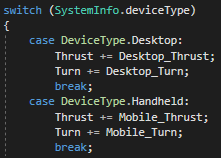
\includegraphics[width=0.6\linewidth]{images/inputdelegate}
  \caption{Dynamic input handling}
  \label{fig}
\end{figure}
As seen in Figure 4, Unity API provides an enumeration whose contents can be checked against the \textbf{SystemInfo.deviceType} value and the \textbf{Thrust} and \textbf{Turn} delegates are assigned to the proper implementation. This way the device specific code can be decoupled from the generic, common game components, enabling smooth and simple transition from one platform to the other. \\ 
In the case of a space shooter game, often times the Acceleration and Deceleration mechanics are considered unnecessary. In our sample game, those have been implemented for PC only, as it facilitated the presentation of various game data. On the Android platform, the player ship will always move with maximum velocity. \\ \\
After another glance at Figure 2.b, there is another UI element to be noticed, the two bars in top left, red and cyan. These are responsible for the survival mechanics. Red represents the ship's hull (health), while cyan represents the ship's force field (shield). Upon collision with an asteroid or an enemy projectile, first the shield is depleted, and then health points are deducted. The game ends when health points reach zero. While actual values are not displayed, they are proportionally reflected in the fill percentage of each bar. These bars, as UI elements, do not directly interact with other game objects, instead their attached scripts adjust the fill rate based upon player status data. \\
The asteroid field is composed of up to 2048 asteroids. They are initially created in a grid of 8 x 8 x 8, with minor random deviations to each axis. Each asteroid slowly moves on its set trajectory, which is also random. An asteroid can be destroyed by repeated projectile hits, or by collisions with other asteroids, drones or the player ship. Upon destruction, an asteroid breaks into two smaller asteroids, which also break into two yet smaller ones. These smallest asteroids do not break into smaller pieces, instead simply exploding upon destruction. \\
The space drones are static, up to 15 of them are randomly placed in the asteroid field. They will continuously rotate to face the player ship, and fire as often as possible. The space drones do not possess any movement mechanics, and do not have a shield. 
\subsubsection{Effects}
Multiple visual effects can be found in Space Shooter. The most notable one is the force field effect around the player ship. This shield is in fact a sperical particle system, with particles projected on a virtual sphere to give it an animated look. A transparent material is applied to this sphere, and randomly generated noise that provides the blurring effect across a slightly colored hue. The particle system has a pulse effect, with a frequency of roughly 0.7 seconds caused by the particle emission. This phenomena occurs because that's how long a particle emission cycle lasts in this particular effect. The particle system will continuously loop, giving the impression of a continuous bubble, which only stops when the player's shield points reach 0. Once they regenerate sufficiently, the shield will reactivate along with its particle system. \\
The shield has an additional visual effect, upon collision with other objects. The collision triggers a new shader effect, which sends additional noise across the spherical surface, as a shockwave ring moving away from the point of impact. \\ \\
Another effect is the engine trail on the player ship. It is based on Unity's Trail Renderer, which functions similarly to a particle system, except instead of particles being constantly thrown out, they are left behind as the object is moved around the game world. The pefromance impact of trail renderers is quite small, but they are often paired with Point Ligth objects when creating propulsion effects. A similar effect, without extra light, is used for the player weapon projectiles, to facilitate lighting while making the game a little more spectacular.\\
 Light sources in the game can be a dangerous tool. They bring life to a game scene, but, depending on configuration, they can be costly to process. Like everything in a game, light is not real, and must be simulated. But depending on the choice of rendering, and of desired fidelity, lighting can be one of the harshest things to process in a game. In this case, it is a single point light that only casts very simple shadows. \\ \\ 
 The last major effect to be noted in the game is the explosion. Whenever something in Space Shooter is destroyed, it explodes, whether it is an asteroid or a drone. They are classical one-shot particle systems, using many, fiery colored particles that launch in a quick, expanding, burst, and imploding afterwards. This effect can potentially bring high performance penalties to the game, depending on how it is implemented. \\ \\
 As a conclusion regarding Space Shooter, there are a lot of basic tools present in Unity, basic but powerful, with which a content creator can make fascinating effects. In the next secions we will discuss the real-world aspects of game development, how to measure a game's performance and then improve it.
\subsection{Performance testing}
Performance tests determine how fast the system or some parts of the system can work under the particular workload. Load testing, stress testing, configuration testing, spike testing are some of the sub categorization of performance testing. \cite{testingarticle} \\ \\
Unlike specialized software, a game can greatly benefit from its availability on as many devices as possible, thus facilitating the highest player base possible. As an example, many productivity tools could prove a cumbersome experience when used on a smartphone, such as Autodesk products, while a game available on mobile devices enable users to play it everywhere, providedthat suitable means of input are implemented. According to the Cambridge Dictionary of English, a game is defined as `` an entertaining activity, esp. one played by children, or a sports competition'' \cite{gamedef}. As an entertinament source, games cannot therefore be considered critical applications, providing great flexibility in regard to specifications. \\ \\
Performance analysis in games may not exclusively be used to prove that the product complies with specifications, but also to identify headroom. If performance is way above expectations, the game could be a candidate for availability on lower performance platforms that were not previously considered. Unity's cross-platform development solution makes this relatively easy by allowing the developer to create platform specific quality settings, as will be discussed later on in this paper.\\ \\
When the gameplay experience is not stable and constant, measures must be taken to address this issue. When tracking the game performance during development, a consistent test environment is needed to ensure results are not biased by external factors (a more powerful machine may yield better results despite a later version actually performing worse than the previous one tested on a slower machine). Thus, when preparing for tests, all the teams should update their code, tests, documents and test environment and align them \cite{gamedef} to ensure consistent results.
The following subsections will present the methodology and environments used to test Space Shooter. Being a purely demonstrative application for key consepts, the game has no product documentation, nor does it have specifications. Testing will be focused only on the performance of the existing application, in its current form, and the changes caused by the implementation of the techniques discussed in future sections.
\subsubsection{Test environments}
As previously stated, consistent testing environments are of critical importance to ensure the relevance of the results following a test over successive iterations of an application. Space Shooter is being developed on the Windows PC platform, and is aimed to also run as an Android application. As such, for the demonstrations required by this study, one Motorola Moto E4 was considered a good choice, both because of availability reasons, as well as the fact that its specs are on the lower end of the performance spectrum compared to premium, latest gen devices. This way, every performance gain, however small, will have a strong impact, especially if the initial gameplay experience is undersirable due to performance issues. \\
Since a Windows PC is used to develop the game itself, we decided to include this machine in the performance test, to see the high-end spectrum as well. Performing the same tests on a computer that can already run the application much better than needed may yield interesting results and surprising insights. Both devices capabilities can be found in the previously shown Table 1, under the ``Moto E 4'' and ``Custom-built PC'' entries. \\ 
Both devices will run the latest relevant updates (drivers, operating system updates) during the start of the process, and they will not be further updated in case of future releases for the sake of consistency. 
\subsubsection{Measurements}
Like other forms of computer graphics, the game is rendered as a rapid succession of images, rapid enough that the human eye perceives continuous movement. These images are called framerates, and the speed at which they are displayed is referred to as framerate, measured in a second, and called Frames Per Second or FPS. \\
According to a York University research in partnership with others, in all conditions tested, there was a clear preference for higher frame rates (48fps and 60fps) when contrasted with a standard of 24fps, regardless of content. \cite{fpspaper}. And while the transition from 48 to 60 FPS was not always showing improvement in general, the study also shows that, when dealing with high-action scenes with rapid movement, the preservation of the illusion of movement offered by increased framerates has a noticeable impact on the viewer. \\ \\
Given these facts, the framerate proves to be a reliable and relevant means of measuring a game's performance across various platforms. An initial goal of 24 FPS will be aimed for, and for a hypothetical mobile release, the framerate will be limited to this value to preserve battery life in a mobile device. For the purpose of testing however, we will attempt to reach higher values if possible. \\
Given that mobile devices are not meant for multitasking, we will not be too concerned about resource usage otherwise, provided the device has sufficient resources to run the game in the first place. Should this not be the case, the framerate will be considered zero.
\subsubsection{Testing methodology}
Because of the risk of interference from background processes competing for resources, each test will be repeated five consecutive times. During each test, the current framerate will be sampled every second and stored for the end results. Tests must contain all types of content available in Space Shooter except the defeat screen which is a trivial scene. The test data will be collected for a period of 30 seconds of play time. This value has been considered appropriate to the game's relative simplicity and will be enforced by adding an automatic game ending timer set for this period of time.\\
Content types are:
\begin{enumerate}
\item Moving towards empty space (no asteroids)
\item Moving towards the asteroid field
\item Destroying an asteroid with the ship weapon
\item Destroying a drone with the ship weapon
\item Destroying an asteroid through collision
\item Get hit by drone weapons several times
\item Lost and regenerate ship shield
\end{enumerate}
Once all five tests are completed, the data from all will be combined. The combined data will then be compiled into the following information:
\begin{enumerate}
\item The mean framerate across the runs
\item The standard deviation of the framerate
\item The mean of the top 10\% of the entries
\item The mean of the bottom 10\% of the entries
\end{enumerate}
The mean value across all samples provides the baseline for performance. It is the general value that tells us how the game performs overall. However, a high mean value may prove insufficient, as a potential bad practice during implementation may drastically lower performance of one component that is not present with high frequency and thus having a relatively small influence over the result. \\
The standard deviation will indicate how stable the result is performance-wise. Ideally, everything is properly optimized and has a similar cost, therefore the framerates stay constant throughout the gameplay, indicated by a deviation value close to zero. On the other hand, if a particular game component is particularly slow, the framerate will dip by a big margin and will increase the standard deviation to reflect this imbalance. \\
The top and bottop 10\% means are used to further identify extremes. A top 10\% mean close to the overall mean means the game is mostly optimized, as the majority of components performs quite similar to those that are relatively fast (it is highly improbable that every single game component and scenario is highly complex and inefficient, which would in any case be identified by a very low global mean). The bottom 10\% mean is used to identify how much worse the lower performing components operate compared to the rest. By constantly working to optimize the game aspects responsible for the bottom 10\% values, this value can be raised, decreasing the standard deviation and increasing the mean. In a real-world scenario, this process would be repeated incrementally until optimal results are met.
\section{Improving performance}
The scale of the performance topic in computer applications is extremely broad, and beyond the scope of this article. In this chapter, we will focus specifically on Space Shooter, and on certain techniques for improving it, along with measuring the gains that come with their implementations. These implementations will be progressive as opposed to being implemented separately, on the same base application. This decision was made in order to better reflect a real process of optimizing a game.
\subsection{Quality compromises}
The most straightforward method of improving a game's performance is to simply cut some content, or lower the quality of some aspects. It consists of many small changes, that together may (hopefully) have a noticeable impact. The game should be analysed against the target platforms. Perhpas the resolution of some textures is too high for a target platform, or perhaps the game world can be reduced in scale. Unity provides a great tool for managing quality, enabling the developer to create Quality Settings profiles for the project. These can affect and overwrite certain effect specific settings, and can be freely distributed across target platforms. Texture resolution can be decreased from the original, high-quality texture, shadow and rendering improvements such as Anti Aliasing can be reduced, or disabled altogether, without impacting other platforms. A study released by the Hindawi Publishing Corporation confirms that visual quality of an image relies not only on the image itself, but is also closely tied to the characteristics of the screen displaying them. Resolution, pixel density, screen size, all influence and potentially bottleneck the quality of the image that the end-user will see. \cite{imgquality}. \\ \\
The original Space Shooter comes with full quality of all its assets. The original skybox texture has a 4k resolution, and the game world consists of 512 asteroids and 30 hostile drones, continuously firing towards the player. All special effects, such as particles, will be left as created, with visual quality as a priority. \\
One aspect to note, a traditional game development technique has already been implemented, because the other option was not only cumbersome to implement, but also highly inefficient on both development time and resources. The asteroid field consists of only 4 distinct asteroid models, slightly altered in scale by randomized deltas. Having 512 distinct asteroid models is both a daunting graphical design task, and non-scalable for increasinly big fields. As such, one useful technique is Model/Texture Sharing. With a small, yet sufficiently large pool of assets, an illusion of diversity can be created that is indistinguishably close to real diveristy during play time, but with a fraction of the resources needed.
Another quality setting that affects performance is Anti Aliasing. Because 3D objects are rendered in a game as a mesh of triangles, sometimes the shapes are rendered with jagged edges. Anti Aliasing addresses this, but through a relatively expensive computational process on the GPU. The effect however seems less severe on a smaller screen, therefore it may be useful to remove this effect altogether in the Android release of the game. As stated in the presentation attached to this article, mobile gaming is not aimed to directly compete with ``bigger'' platforms such as PC or consoles, but as an ``on the go'' option. 
High-quality shadows and reflections can also negatively influence a game's performance, and may grow unnoticed in a high-action game. The traditionally used rendering method, rasterization, already uses light maps for an approximation of realistic shadows, and as a time-tested method, an indication that perfect simulation of reality is often not necessary for an enjoyable gaming experience. Unlike the state of the art real time ray tracing technology released in August 2018 by Nvidia, rasterization is much less computationally intensive, but even so, without optimizations, a game can be quite difficult for hardware to run within acceptable parameters. \\ \\
In an attempt to optimize the game based on the previously mentioned methods, the following changes have been done to Space Shooter in an attempt to improve the performance:
\begin{enumerate}
\item{Skybox texture base resolution has been reduced to 1k, from 4k}
\item{Rendering resolution of the skybox texture has been reduced to one eighth of the base resolution}
\item{Enemy drone count has been reduced to 20, down from 30}
\item{Asteroid count has been reduced to 216, down from 512}
\item{Explosion particle count and emission rate have been greatly reduced}
\item{Anti aliasing has been completely removed}
\item{Shadows and reflections have been disabled}
\end{enumerate}
The results are quite interesting. The framerate in the unoptimized games has been quite even, except for the spikes associated with restarting a level and reinitalizing the game world to the original state. Figure 5 shows the framerates across the 5 tests pre and post optimizations for both platforms, and we can see that especially on PC (Android as well, but less so), the framerate has high fluctuations, but overall is in a higher value range than before. Table 2 shows even more details. Overall, there has been a 133.44\% improvement on PC, but the standard deviation has increased over 5 times. This indicates that there are other components of the game that would require further optimization. Looking at the Android values, they seem less impatctful when looking at the graph. With only 14.56\% improvement post optimization, the standard deviation is still significantly higher, by a magnitude greater than 3. This further enforces the hypothesis that while results are better, further optimization areas need to be found. Looking at the minimum values on the Android device, we notice that they are unchanged, at 10. This would indicate that a specific resource is extremely heavily used, and proving a main bottleneck factor.
\begin{figure}
\begin{subfigure}{0.49\textwidth}
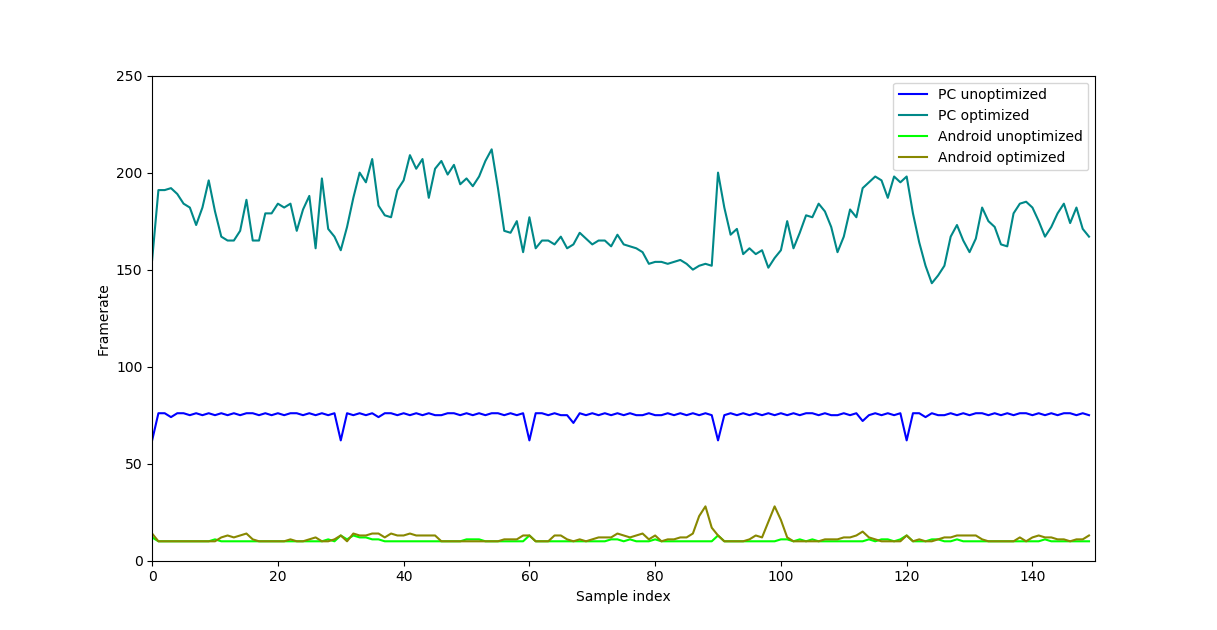
\includegraphics[width = \textwidth, height = 0.66\textwidth]{images/compromise}
\end{subfigure}
\caption{Framerate before and after optimization}
\end{figure}
\begin{table}
\caption{Optimization data}
\label{tab:conf}
\begin{minipage}{0.49\textwidth}
\begin{center}
\begin{tabular}{lllll}
Value & PC pre & PC post & Android pre & Android post \\
Mean & 75.00 & 175.08 & 10.30 & 11.82 \\
Std & 2.51 & 15.68 & 0.67 & 2.75 \\
Top 10 mean & 76.00 & 205.50 & 12.30 & 19.40 \\
Bottom 10 mean & 67.50 & 150.50 & 10.00 & 10.00 \\
Min & 62 & 143 & 10 & 10 \\
Max & 76 & 212 & 13 & 28 
\end{tabular}
\bigskip
\end{center} 
\end{minipage}
\end{table}
\subsection{Implementation strategy improvements}
Implementation strategies are highly dependant on the programming language and game engine used. It requires good knowledge of both for effective results. One observation done during previous runs is a noticeable improvement in framerates while the shield is down. Because of extensive usage of shader properties and particles, one attempt at optimization will be creating a similar, simpler force field effect, that will be dynamically chosen at runtime, in case of Handheld devices. The choice between the two effects can be done when initializing the game scene, thus having no impact during the actual gameplay, save for the benefits of a simpler effect in case of a handheld device.  \\
Dickinson strongly discourages the usage of Draw Calls on mobile platforms, specifically related to high material counts, as well as alpha testing. It is therefore recommended to reuse as many materials as possible, with preferably square sized, low size textures, which will also improve VRAM and Memory Bandwidth usages. For example, the iPhone 6S could only support texture sizes of up to 2048x2048. \cite{optimizationbook} In Space Shooter, due to the low performing hardware used, all textures will be reduced to 256x256 sizes. This optimization may be considered as fitting under the Quality Comporomises section, but due to the subtlety of knowledge involved, it was decided it fits better here. \\ \\
An additional, minor improvement, is going through each of the scripts, and removing the autogenerated methods. Each class derived from Unity's MonoBehaviour will have a number of callback functions defined empty. At runtime, when the MonoBehaviour class is instantiated, all the implemented methods will be hooked, regardless of it being empty. Some of these functions (such as Update, called every frame, for every object, or OnCollisionEnter, in the presence of a RigidBody) can add an overhead that keeps adding up, slowing down the CPU side of the processing. \cite{optimizationbook} We will attempt at removing and avoiding all unnecessary function definitions, and ensure that actions that only need to be taken once are placed in the right function, for example the dynamic choice of force field effect should be done during the call to Start or Awake, which only execute once, during initialization, instead of the Update function.
Figure 6 shows the results of further optimizing Space Shooter, after the previous section. On the PC, the differences are very subtle. The mean values are so close, 175 to 179, that it could be attributed to background interference. However, a slightly increased mean, and a slightly decreased standard deviation would suggest a minor uniformization of the framerate, which is one of the goals. \\
On the mobile side of things, the results are a little better. The average framerate shows a 35.44\% improvement, with an approximate 130\% increase in standard deviation. While the minimum, maximum and bottom 10 average are mostly unchanged, we can see that along with the higher standard deviation, the top 10 mean is also showing an increase of almost 45\%, suggesting that likely textures were one of the contributing factors. \\ \\
\begin{figure}
\begin{subfigure}{0.49\textwidth}
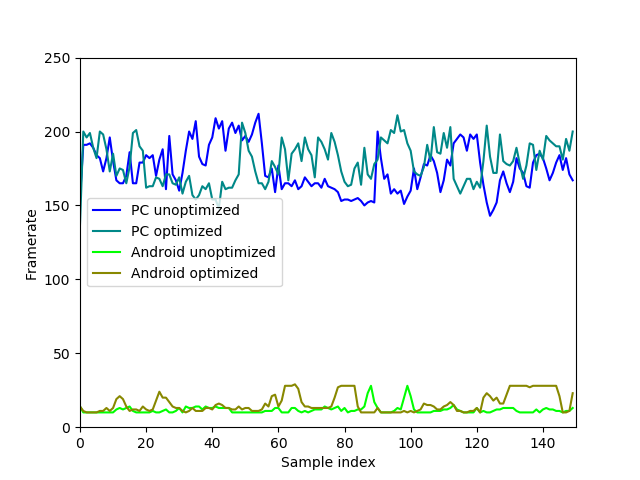
\includegraphics[width = \textwidth, height = 0.66\textwidth]{images/general}
\end{subfigure}
\caption{Framerate before and after optimization}
\end{figure}
\begin{table}
\caption{Optimization data}
\label{tab:conf}
\begin{minipage}{0.49\textwidth}
\begin{center}
\begin{tabular}{lllll}
Value & PC pre & PC post & Android pre & Android post \\
Mean & 175.08 & 178.94 & 11.82 & 16.01 \\
Std & 15.68 & 14.40 & 2.75 & 6.32 \\
Top 10 mean & 205.50 & 203.00 & 19.40 & 28.10 \\
Bottom 10 mean & 150.50 & 153.80 & 10.00 & 10.00 \\
Min & 143 & 137 & 10 & 10 \\
Max & 212 & 211 & 28 & 29 
\end{tabular}
\bigskip
\end{center} 
\end{minipage}
\end{table}
While we have seen no dramatic increase in numbers with any of the optimizations so far, comparing Figures 5 and 6, we have improved the performance of the game by around 50\%. Ideally, the numbers can be pushed higher by further optimizations, and reaching the goal of a stable framerate, averaging at least 24 frames per second, the minimum value for an animated experience, preferably with a small deviation for consistency. \cite{fpspaper}
\subsection{Object pooling}
One aspect of Unity that consumes a lot of processing power and time is the instantiation of game objects from prefabs. Because such objects can have a significant runtime memory footprint, creating and destroying them can become a bottleneck as far as performance is concerned. Dickinson's orc example on page 297\cite{optimizationbook} can be applied to many scenarios regarding temporary objects. For Space Shooter, destroyed asteroids instantiate two lesser ones, and those again spawn another two each, for a potential total of additional 6 instantiations per each original asteroid. On top of this, the player weapon spawns new projectiles every time it is fired. The space drones also continuously fire at the player ship, continuously creating a large number of projectile objects. On top of all these, the destruction of an asteroid or drone is accompanied by an explosion effect, which is also a game object containing a particle system.\\
 All these potential gaps in performance could be improved, by creating object pools. Instead of destroying them only to create new ones later, it would be more efficient to simply disable an object that is not needed anymore, and reuse it when needed again. Depending on a case by case basis, one significant question must be answered: How to deal with an insufficient object pool? For example, in a hypothetical explosion object pool of 30 objects, what would happen in case 31 explosions are triggered at once? \\
 One possible answer is to increase the pool by instantiating an additional one. One instantiation, while perhapes less than desirable, is still much better than 31. \\
 Another option can be simply ignoring the 31st explosion, or to generalize, when there are no available objects in the relevant pool, don't do anything. While this can be the best option when targeting performance, it may have a strong undesired impact over the player's experience of the game. \\
 The third option, the middle ground, is instead to reuse the oldest active object in the pool. While it may also have a noticeable, non constant effect on the player, their attention is likely to be focused on the action at hand, therefore an explosion somewhere in the background may go unnoticed, as opposed to destroying an asteroid and sometimes not triggering anything beside the asteroid disappearing and two smaller ones appearing in its place. \\ \\
 It is important when creating an object pool to determine a good estimate of its size, to preserve a balanced memory usage. In the case of Space Shooter, we can determine that since each original asteroid will break into two, and the two pieces will break into another two, the maximum number of asteroids that can be at any one time is four times the original number. However, if the asteroid pool would be initialized with the maximum count, it is very likely that many of the pooled object will remain unused. After experimenting with different values and monitoring the creation of new Asteroids when needed, we have chosen an initial pool 35\% larger than the initial count. With this value we do not have a very high overhead, and extremely rare occurences of additional objects needed. \\
 In regard to the explosion pool, the maximum possible number of instances at any one time would be the maximum possible count of objects that can trigger an explosion. It would be therefore four times the original asteroid count, plus the space drone count. This would be a much too great number of objects to pool, especially for a purely visual component. We will therefore initialize the pool with a static count of 20 explosions for asteroids, and 5 for drones, and reuse the oldest active explosion if there are none available. \\
 The projectile maximum count can be calculated by dividing the lifetime of the projectile with the fire rate of the weapon, adding one, and multiplying the result with the total count of weapons, calculated separately for each weapon. Because weapon fire should be a reliable game mechanic, we will initialize the projectile pools with the optimal number of projectiles, as reaching the maximum count can be a relatively easy to encounter situation.
\section{Conclusions}
In this paper we have looked at several means of improving and stabilizing the performance of a sample game implemented in Unity. While the end results may not be called extreme, significant improvements can be seen between the initial and final reading as per table 5. Looking again at the first and last values, using a few basic techniques, Space Shooter has gained more than doubled the average framerate on PC with extremely similar deviations, and the Android version was improved by over 91\%, albeit with more fluctuations. \\
Looking at the rest of the entries, we can see that the previous statements hold true, with extremely similar changes between the original and optimized version of the game.
``The one constant cost included in all performance optimization work is time. So, with
limited time at our disposal to both implement the features we want to implement and keep
everything working, an important skill to learn for any developer is workflow optimization.
Better understanding of the tools we use will save us more time in the long run, and
hopefully provide the extra time we need to implement everything we want to, which
applies not only to the Unity Engine, but to every tool we use.''\cite{optimizationbook}
\begin{table}
\caption{Optimization data}
\label{tab:conf}
\begin{minipage}{0.49\textwidth}
\begin{center}
\begin{tabular}{lllll}
Value & PC pre & PC post & Android pre & Android post \\
Mean & 75.00 & 155.04 & 10.30 & 19.70 \\
Std & 2.51 & 2.77 & 0.67 & 7.12 \\
Top 10 mean & 76.00 & 159.20 & 12.30 & 28.60 \\
Bottom 10 mean & 67.50 & 150.30 & 10.00 & 10.00 \\
Min & 62 & 146 & 10 & 10 \\
Max & 76 & 160 & 13 & 29 
\end{tabular}
\bigskip
\end{center} 
\end{minipage}
\end{table}
\begin{acks}
This work was carried out within the Web and Mobile Apps class. \\
Credits to QINE, IGGY-DESIGN, PIXEL MAKE and NIGHTSOUNDGAMES for their visual models and effects available on the Unity Asset Store, that were used to develop Space Shooter. \\
A lot of inspiration regarding optimization techniques within Unity has been found in the Unity 2017 Game Optimization book written by Chris Dickinson (Packt Publishing).
\end{acks}

\bibliographystyle{ACM-Reference-Format}
\bibliography{literature}

\end{document}
